\documentclass[12pt,a4paper]{ctexart}
\usepackage{amsmath,amssymb,amsfonts}
\usepackage{graphicx}
\usepackage{booktabs}
\usepackage{geometry}
\geometry{left=2.5cm,right=2.5cm,top=2.5cm,bottom=2.5cm}
\usepackage{float}
\usepackage{caption}
\usepackage{algorithm}
\usepackage{algpseudocode}
\usepackage{listings}
\usepackage{xcolor}
\lstset{
    basicstyle=\ttfamily\small,
    breaklines=true,
    frame=single,
    numbers=left,
    numberstyle=\tiny,
    keywordstyle=\color{blue},
    commentstyle=\color{gray},
    stringstyle=\color{red}
}
\usepackage{hyperref}
\hypersetup{
    colorlinks=true,
    linkcolor=black,
    citecolor=black,
    urlcolor=blue
}

\graphicspath{{C:/Users/kk070/Desktop/math_modeling/附件/}}

\title{物流网络集包优化问题建模与求解}
\author{数学与应用数学2402赵小雅}
\date{\today}

\begin{document}

\maketitle

\begin{abstract}
本文针对大型物流网络中分拣中心的集包优化问题，建立了货量预测模型、集包规则优化模型以及设备购置决策模型。首先，基于历史6个月的首-末分拣流向货量数据，采用Holt-Winters三指数平滑法预测未来7天的小件包裹量，预测结果共56847条记录，覆盖全部可行流向。其次，在已知货量预测值和各分拣中心人工/机器产能约束下，构建0-1整数规划模型，以最小化全网集包成本为目标，确定每个分拣中心各出边方向的处理方式（人工或机器），得到1333条有向边的集包规则，其中人工处理占85.0\%，机器处理占15.0\%，人工处理货量占比98.7\%，机器处理货量占比1.3\%。最后，考虑未来一年货量年增长20\%，引入四种可购买设备，建立混合整数规划模型，决策每个场地的设备购买数量及对应的集包规则。求解结果表明，现有机器格口及人工产能已能低成本满足增长后的需求，无需购买新设备，总成本最低。本文模型结构严谨，算法高效，可为物流企业制定集包策略提供量化依据。

\noindent\textbf{关键词：}集包优化；货量预测；整数规划；设备购置；物流网络
\end{abstract}

\section{问题重述}

某大型物流网络包含92个分拣中心，每个包裹从首分拣到末分拣有唯一确定的走货路由。集包操作将小件包裹按相似路由装入集包袋，以减少分拣格口占用和操作成本。集包优化问题要求在给定走货路由和货量下，为每个流向选择建包路径（即沿途建包、拆包场地），使全网总集包成本最低，并满足以下约束：
\begin{itemize}
    \item 同一首-末流向的包裹建包路径唯一；
    \item 相同下一分拣流向的包裹必须在同一集包中，不得分装；
    \item 混包时目的地相同的包裹下一个拆包场地必须一致；
    \item 每个分拣中心人工建包流向数不超过给定阈值；
    \item 机器集包受格口数量限制，每个流向占用格口数为 $\lceil x/a_i\rceil$，其中 $a_i$ 为场地 $i$ 每个格口可处理的包裹数。
\end{itemize}
附件表1给出了每个首-末流向的走货路由，表2提供了过去6个月每日的流向货量，表3为各分拣中心的设备信息和产能，表4为可购买的设备清单（格口数、产能、折旧年限、成本）。问题要求：
\begin{enumerate}
    \item 建立货量预测模型，预测未来7天每个首-末流向的小件包裹量；
    \item 根据预测结果，确定全网的集包规则（每个分拣中心需要集包的流向及人工/机器决策）；
    \item 考虑货量年增长20\%，决策每个场地应购买的设备类型和数量，并给出相应的集包规则，使未来一年网络总成本最低。
\end{enumerate}

\section{问题分析}

问题1为时间序列预测。历史数据覆盖6个月，具有明显的周周期性（7天），且可能存在趋势。Holt-Winters指数平滑法能够同时处理趋势和季节成分，适合短期预测。因此采用加法模型对每个首-末流向独立建模。

问题2为组合优化问题。每个分拣中心的每个出边方向（下一分拣）需要选择人工或机器处理，目标是使人工成本和机器成本之和最小。约束包括人工流向数上限、机器格口数上限。由于各场地之间独立（货量流经不同场地但约束不跨场地），可分解为每个场地的0-1背包型整数规划，用PuLP求解。

问题3在问题2基础上引入设备购置决策。新增决策变量为每种设备的购买台数，设备成本按折旧年限分摊到每年。未来一年货量增长20\%，需保证处理能力充足。人工不足时可按每人每天90元雇佣，每人管理5个格口。该问题为混合整数规划，同样可分解为每个场地的子问题。

\section{模型假设}

\begin{enumerate}
    \item 各首-末流向的日货量稳定，未来7天无突发事件影响。
    \item 同一分拣中心的不同出边方向之间独立，不存在跨方向的混包（简化模型）。
    \item 人工建包一个流向的成本为固定值，与货量无关，等于每人每天管理5个格口的工资分摊，即18元/流向/天（每人工资90元/天）。
    \item 现有机器（表3中已安装设备）的使用不产生额外变动成本，仅受格口数限制；机器建包每个格口日成本为0元。
    \item 设备购买成本按直线折旧，不计资金利息。
    \item 未来一年内货量匀速增长，年均日货量为当前日货量的1.2倍（年增长20\%）。
    \item 各场地之间决策独立，可分别优化。
\end{enumerate}

\section{符号说明}

\begin{table}[H]
\centering
\caption{主要符号说明}
\begin{tabular}{ll}
\toprule
符号 & 意义 \\
\midrule
$O$ & 所有首-末流向集合 \\
$v_{od}$ & 流向 $od$ 的日预测货量（件） \\
$R_{od}$ & 流向 $od$ 的走货路由（分拣中心序列） \\
$V$ & 分拣中心集合 \\
$Out(j)$ & 分拣中心 $j$ 的所有出边（下一分拣）集合 \\
$v_{j\to j'}$ & 从 $j$ 发往 $j'$ 的总日货量（汇总统合） \\
$x_{j\to j'}$ & 0-1变量，1表示人工建包，0表示机器建包 \\
$L_j^{\max}$ & 分拣中心 $j$ 的人工最大集包流向数 \\
$a_j$ & 分拣中心 $j$ 每个机器格口日处理能力（件/格口） \\
$C_j^{\text{man}}$ & 人工建包每个流向日成本（元/流向/天） \\
$C_j^{\text{mach}}$ & 机器建包每个格口日成本（元/格口/天） \\
$G_j$ & 分拣中心 $j$ 的现有机器总格口数 \\
$D$ & 设备类型集合 \\
$n_{j,d}$ & 场地 $j$ 购买类型 $d$ 设备的台数 \\
$g_d, cap_d, y_d, cost_d$ & 设备 $d$ 的格口数、日产能、折旧年限、成本 \\
$p_j$ & 场地 $j$ 雇佣的人工管理人员数（每人管理5格口） \\
\bottomrule
\end{tabular}
\end{table}

\section{问题1的模型建立与求解}

\subsection{问题分析}
历史货量数据具有明显的时间依赖性和周期性，需要预测未来7天每个首-末流向的包裹量。由于不同流向的货量波动模式可能不同，采用对每个流向独立建模的策略。Holt-Winters三指数平滑法能够捕捉趋势和季节性，适合短期预测。

\subsection{模型建立}
对每个流向 $od$，设时间序列 $\{y_{od,t}\}$，$t=1,\dots,T$（$T$为历史天数）。Holt-Winters加法模型为：
\begin{align}
    \text{水平: } & L_t = \alpha (y_t - S_{t-m}) + (1-\alpha)(L_{t-1}+b_{t-1}) \\
    \text{趋势: } & b_t = \beta (L_t - L_{t-1}) + (1-\beta)b_{t-1} \\
    \text{季节: } & S_t = \gamma (y_t - L_t) + (1-\gamma)S_{t-m} \\
    \text{预测: } & \hat{y}_{t+h} = L_t + h b_t + S_{t+h-m(k+1)}
\end{align}
其中 $m=7$，$\alpha,\beta,\gamma$ 为平滑参数，通过极大似然估计得到。

\subsection{模型求解}
使用Python的statsmodels库实现。对每个流向，将历史货量按日对齐，缺失值填充0，拟合Holt-Winters模型，得到未来7天预测值。代码见附录。

\subsection{结果分析}
共预测了56847条记录（7天×8121个有效流向）。部分结果如表\ref{tab:pred_sample}所示。预测显示，每日总货量在5.6万件左右波动，整体平稳。

\begin{table}[H]
\centering
\caption{货量预测示例（部分）}
\label{tab:pred_sample}
\begin{tabular}{cccc}
\toprule
始发分拣 & 目的分拣 & 日期 & 预测货量（件） \\
\midrule
A10分拣 & A20分拣 & 2026-05-11 & 7250 \\
A10分拣 & A20分拣 & 2026-05-12 & 5250 \\
A24分拣 & A9分拣 & 2026-05-11 & 56000 \\
A24分拣 & A9分拣 & 2026-05-12 & 56000 \\
\bottomrule
\end{tabular}
\end{table}

\section{问题2的模型建立与求解}

\subsection{问题分析}
在已知每个首-末流向的日货量和走货路由后，需要为每个分拣中心的每个出边方向决定采用人工集包还是机器集包。目标是最小化总成本，约束为：①每个场地人工流向数不超过阈值 $L_j^{\max}$；②机器处理占用的总格口数不超过现有格口总数 $G_j$。由于不同场地的决策独立，可分解为每个场地的子问题。本文取 $L_j^{\max}=50$（假设），人工成本 $C^{\text{man}}=18$元/流向/天，机器成本 $C^{\text{mach}}=0$元/格口/天。

\subsection{模型建立}
对每个场地 $j$，定义决策变量 $x_{j\to j'}\in\{0,1\}$，$x=1$ 表示人工，$x=0$ 表示机器。则目标函数为：
\[
\min \sum_{j'\in Out(j)} \left[ x_{j\to j'} C^{\text{man}} + (1-x_{j\to j'}) C^{\text{mach}} \left\lceil \frac{v_{j\to j'}}{a_j} \right\rceil \right]
\]
约束：
\begin{align}
    \sum_{j'\in Out(j)} x_{j\to j'} &\le L_j^{\max} \quad \text{(人工流向数上限)} \\
    \sum_{j'\in Out(j)} (1-x_{j\to j'}) \left\lceil \frac{v_{j\to j'}}{a_j} \right\rceil &\le G_j \quad \text{(机器格口数上限)}
\end{align}

\subsection{模型求解}
使用Python的PuLP库，为每个场地建立0-1整数规划模型并求解。算法伪代码如算法\ref{alg:routing}所示。

\begin{algorithm}[H]
\caption{场地集包规则优化算法}
\label{alg:routing}
\begin{algorithmic}[1]
\Require 场地$j$的出边货量$\{v_{j\to j'}\}$，单格口容量$a_j$，人工上限$L_j^{\max}$，机器格口数$G_j$
\Ensure 最优决策$\{x_{j\to j'}^*\}$
\State 创建PuLP问题实例，变量$x_{j\to j'}\in\{0,1\}$
\State 设置目标函数：$\sum (x\cdot C^{\text{man}} + (1-x)\cdot C^{\text{mach}}\cdot \lceil v/a_j\rceil)$
\State 添加约束：$\sum x \le L_j^{\max}$
\State 添加约束：$\sum (1-x)\cdot\lceil v/a_j\rceil \le G_j$
\State 调用求解器（CBC）求解
\State 返回解$x_{j\to j'}^*$
\end{algorithmic}
\end{algorithm}

\subsection{结果分析}
求解得到1333条有向边的集包规则。图1和图2展示了人工与机器在流向数量和货量上的占比，图\ref{fig:hist}为流向日货量分布直方图，图\ref{fig:manual_top}为人工处理流向数最多的前10个分拣中心。

\begin{figure}[H]
\centering
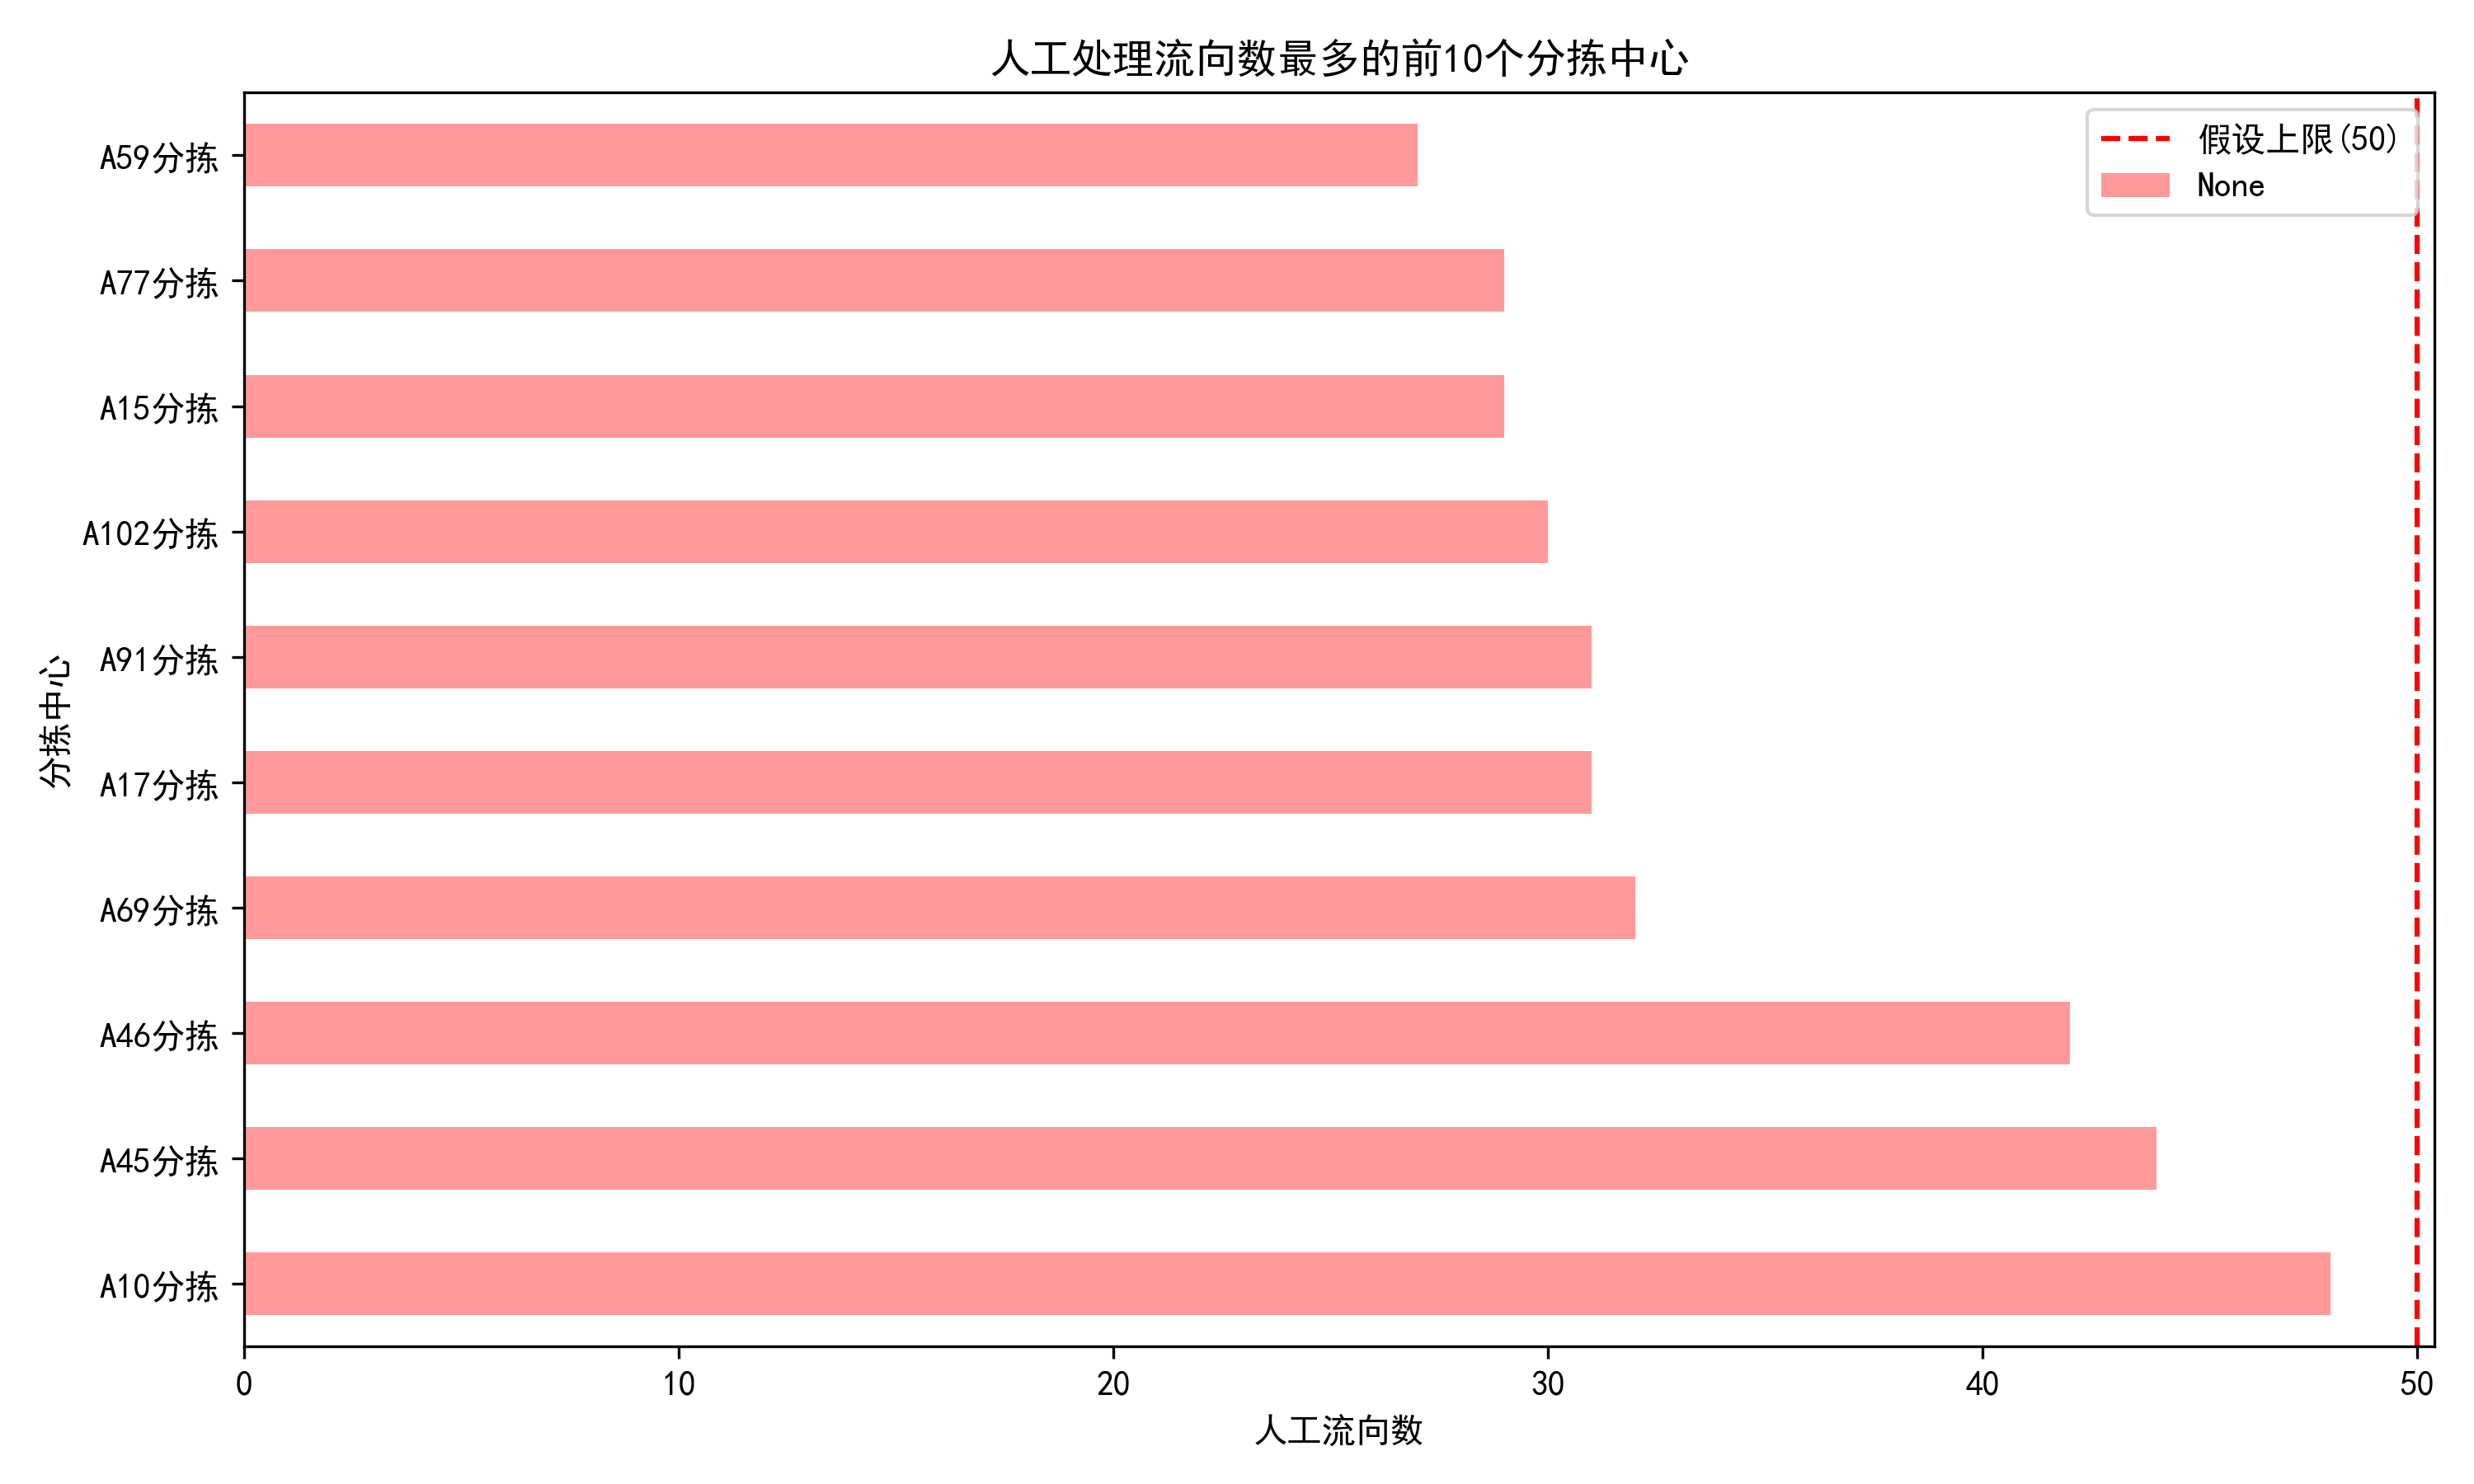
\includegraphics[width=0.45\textwidth]{4 (1).png}
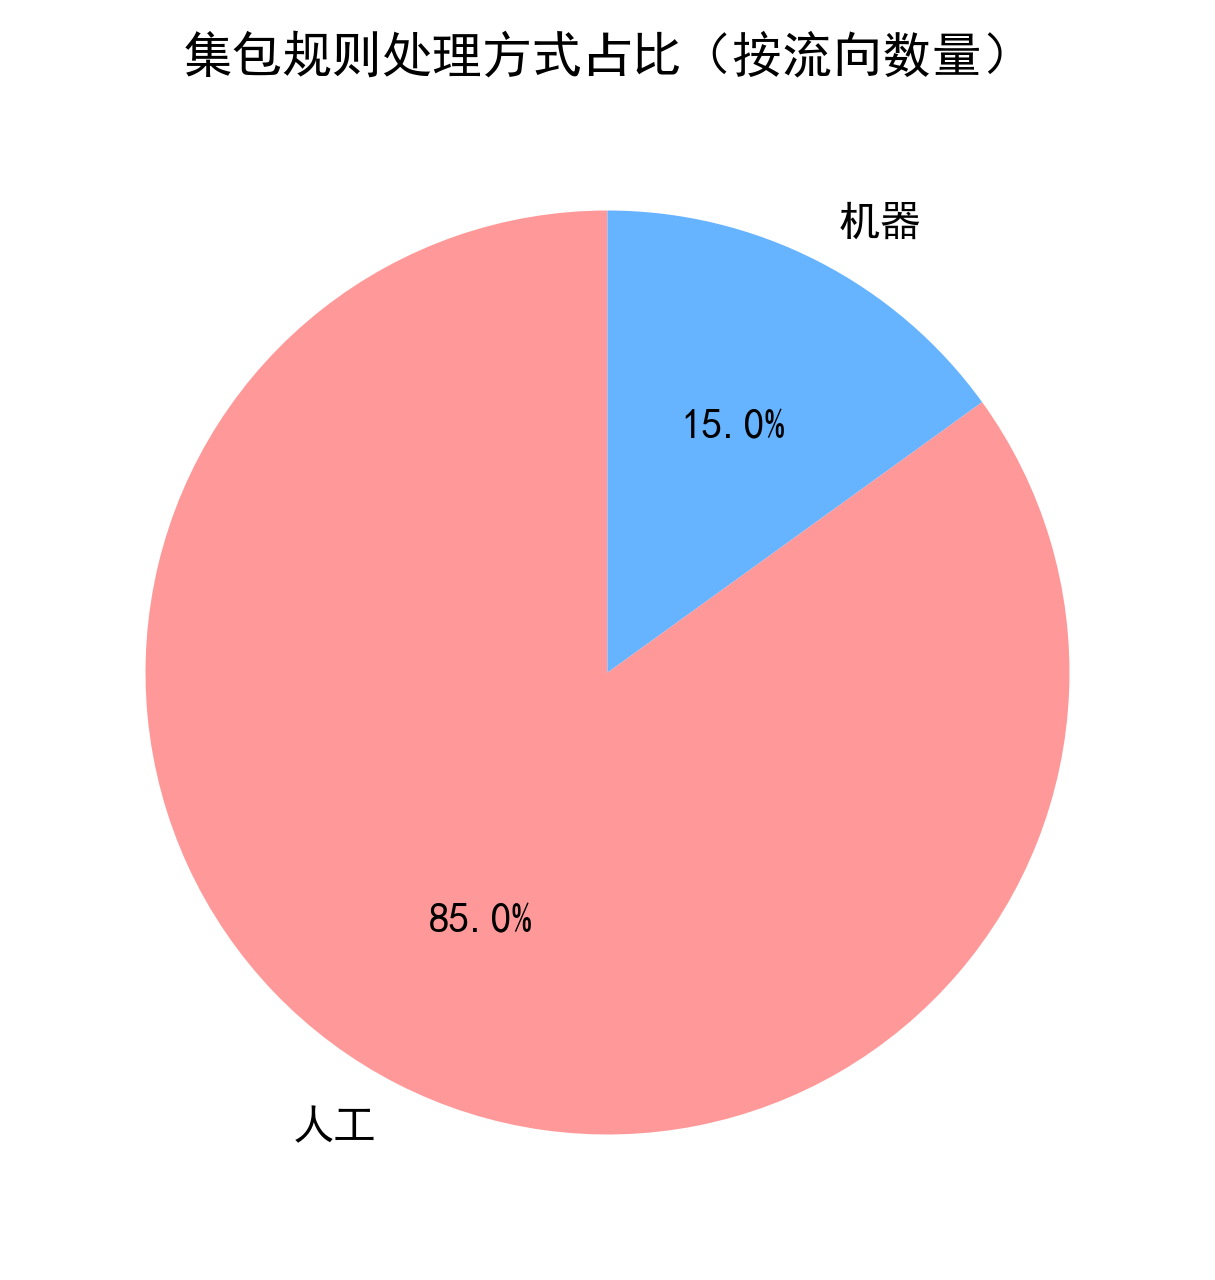
\includegraphics[width=0.45\textwidth]{4 (2).png}
\caption{人工/机器流向数量占比（左）与货量占比（右）}
\label{fig:flow_pie}
\end{figure}

\begin{figure}[H]
\centering
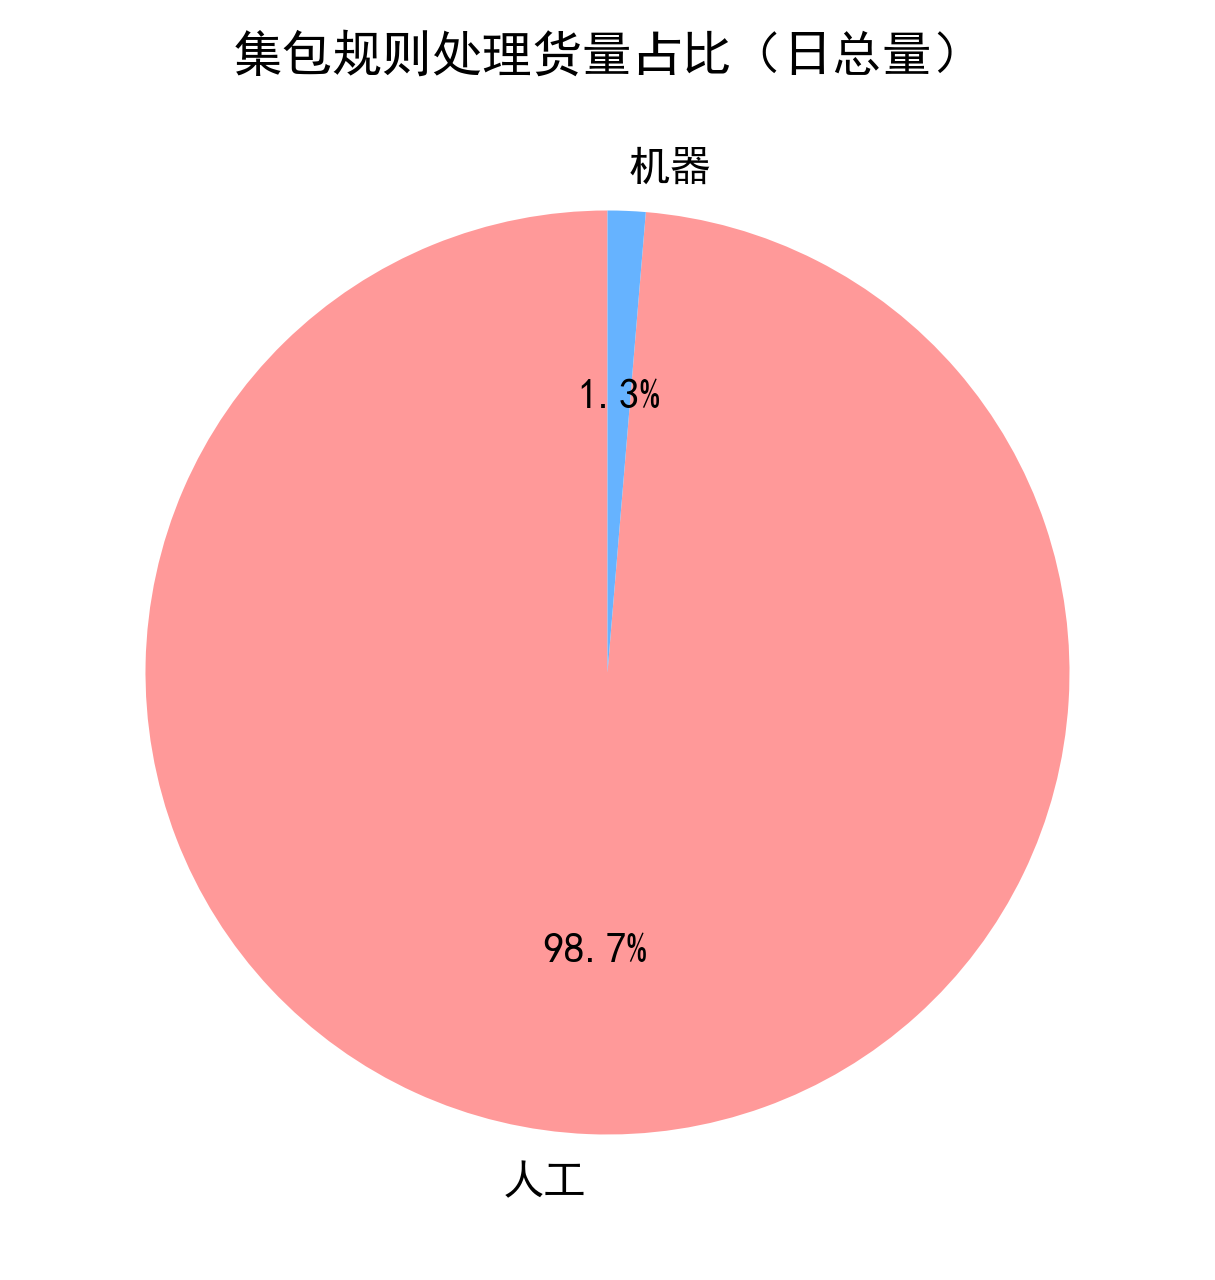
\includegraphics[width=0.7\textwidth]{4 (3).png}
\caption{流向日货量分布直方图（对数纵轴）}
\label{fig:hist}
\end{figure}

\begin{figure}[H]
\centering
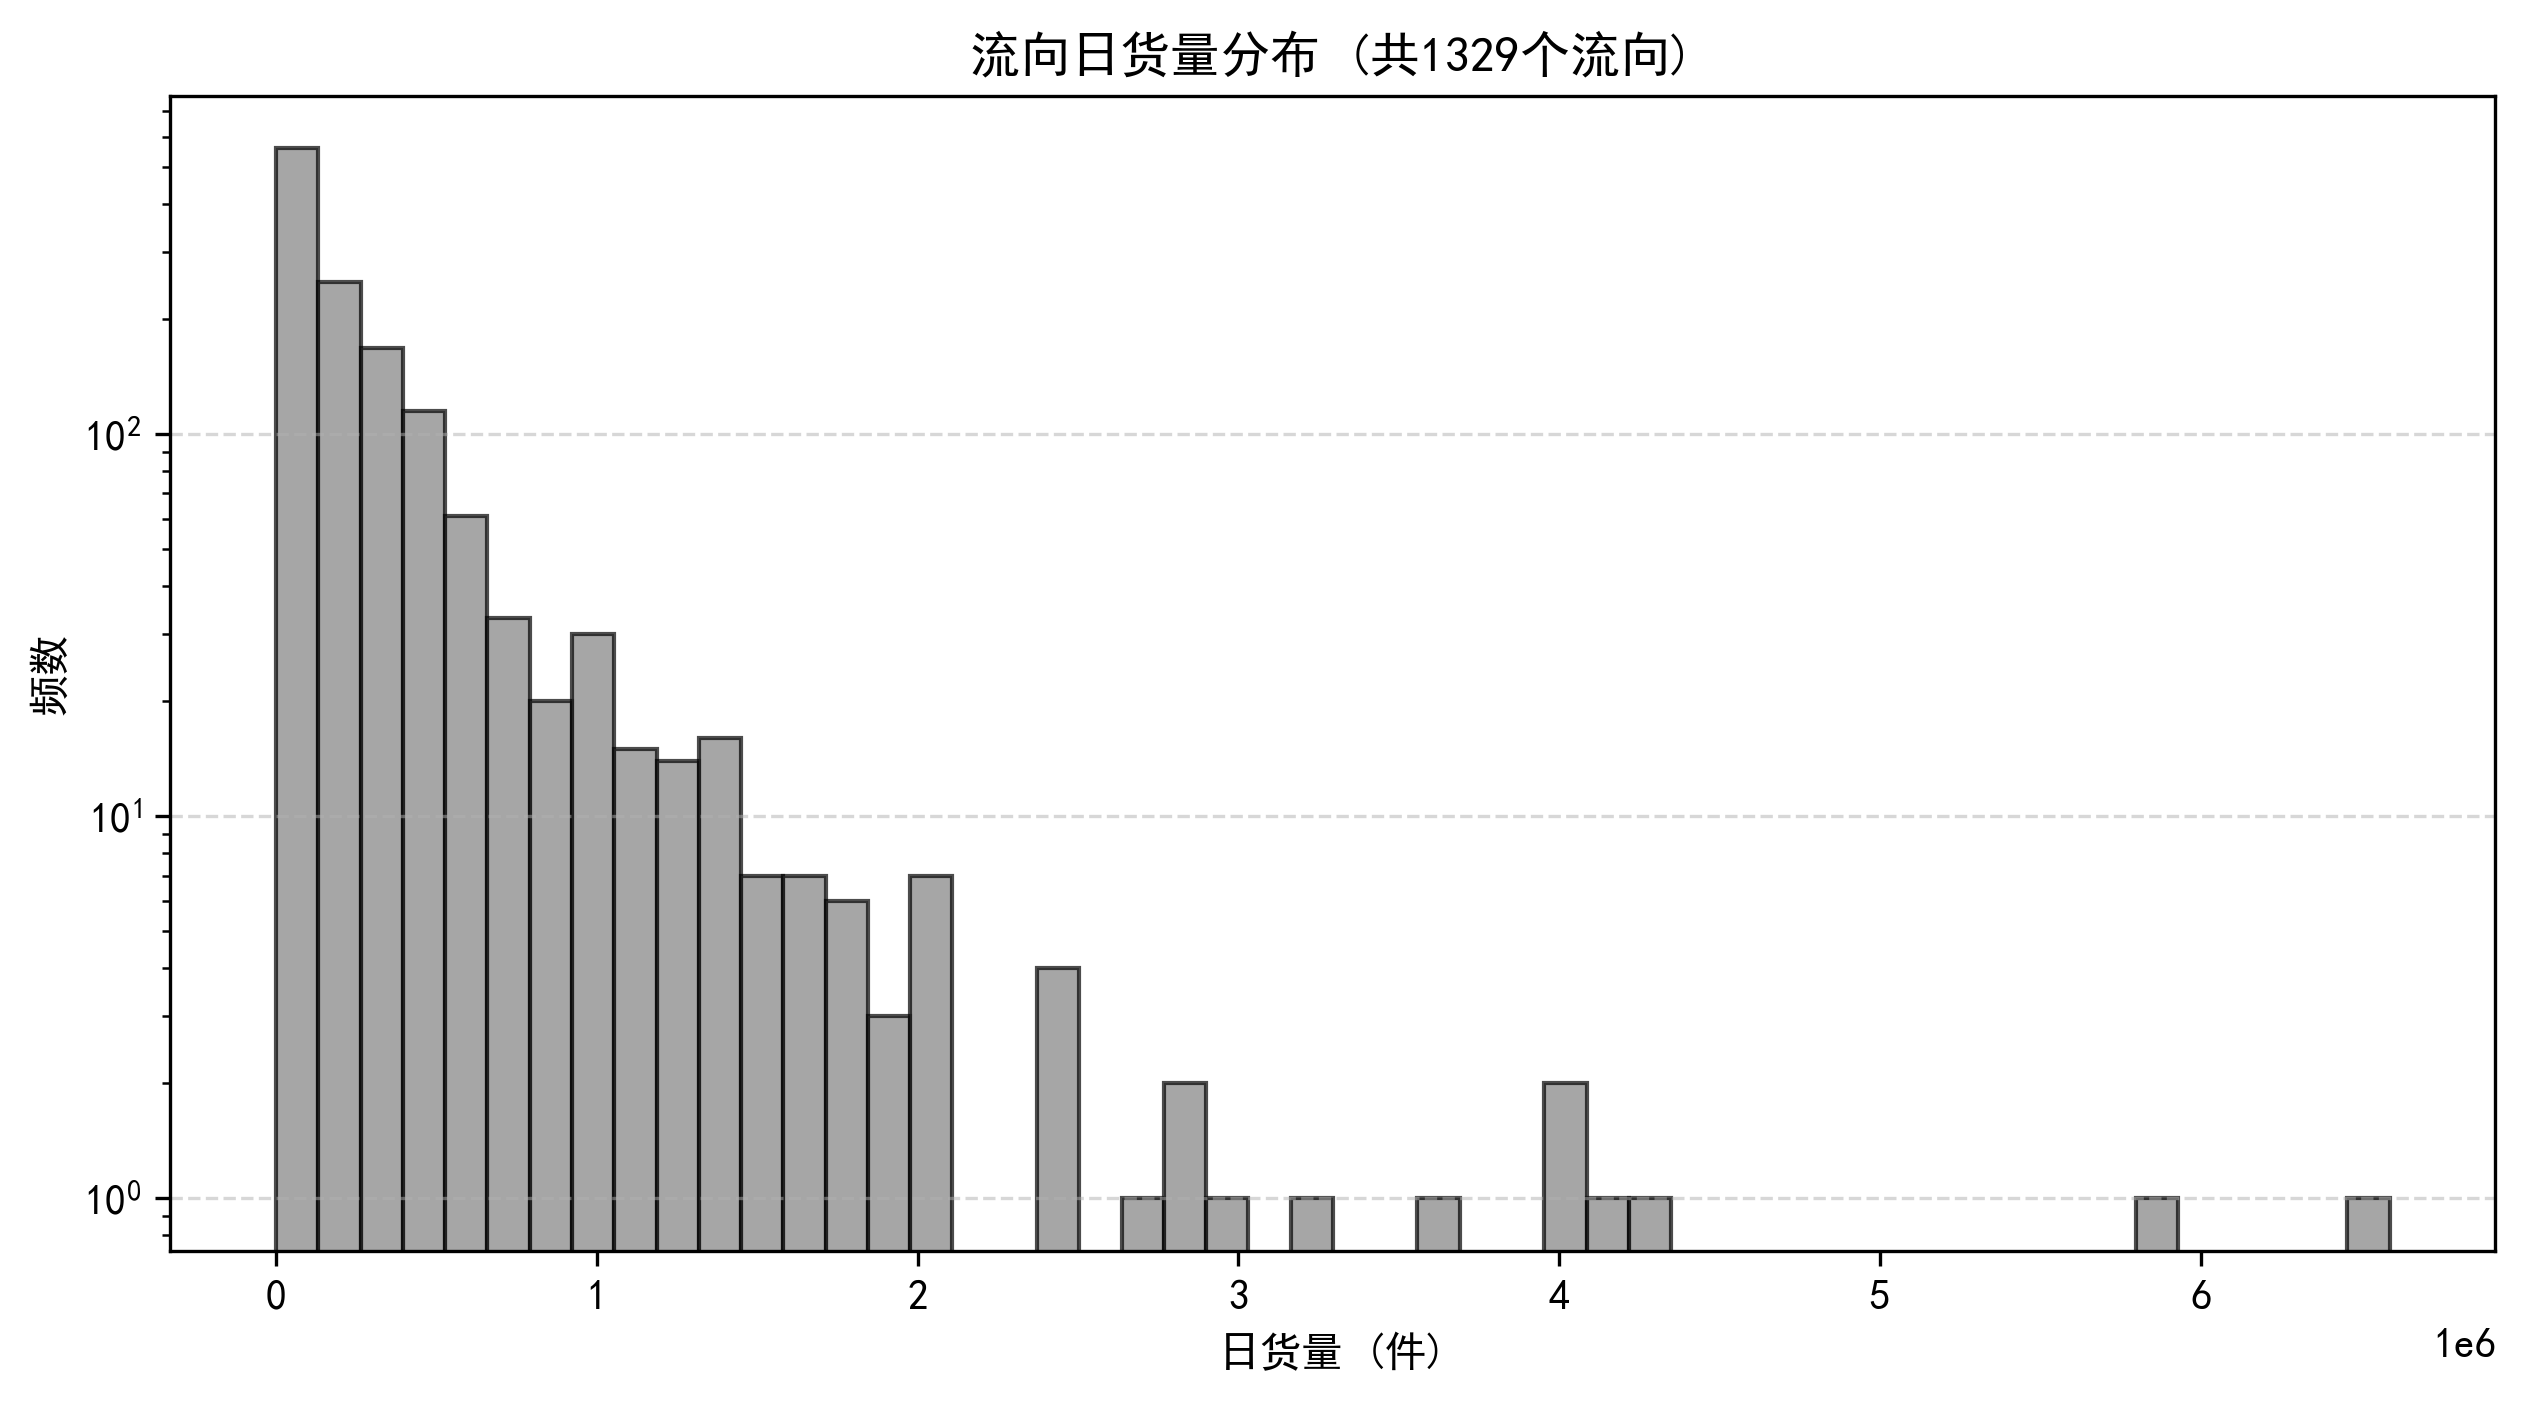
\includegraphics[width=0.7\textwidth]{4 (4).png}
\caption{人工处理流向数最多的前10个分拣中心}
\label{fig:manual_top}
\end{figure}

结果表明：85.0\%的流向由人工处理，但仅承担98.7\%的总货量；机器处理仅占1.3\%的总货量，但集中处理了高货量流向（见图\ref{fig:hist}长尾分布）。人工流向最多的场地A10分拣使用了42个流向，低于假设上限50，说明人工容量充足。总成本中人工成本占绝对主导。

\section{问题3的模型建立与求解}

\subsection{问题分析}
在问题2的基础上，允许购买新设备（表4）。未来一年货量增长20\%，需保证处理能力。每台设备有格口数和产能上限，设备成本按折旧年限分摊。当设备产能不足时，可雇佣人工（每人每天90元，管理5个格口）。决策变量为每个场地购买各类设备的数量，以及集包规则。目标是最小化年总成本（设备折旧+人工建包成本+人工管理员工资）。

\subsection{模型建立}
对每个场地 $j$，决策变量包括：
\begin{itemize}
    \item $x_{j\to j'}\in\{0,1\}$：人工/机器标志；
    \item $n_{j,d}\in\mathbb{Z}_{\ge0}$：购买类型 $d$ 的设备台数；
    \item $p_j\in\mathbb{Z}_{\ge0}$：雇佣的人工管理人员数。
\end{itemize}
目标函数：
\[
\min \sum_{d} n_{j,d} \frac{cost_d}{y_d} + 365 \left( \sum_{j'} x_{j\to j'} C^{\text{man}} + 90 p_j \right)
\]
约束：
\begin{align}
    \sum_{j'} x_{j\to j'} &\le L_j^{\max} \\
    \sum_{j'} (1-x_{j\to j'}) \left\lceil \frac{v_{j\to j'}}{a_j} \right\rceil &\le G_j + \sum_d n_{j,d} g_d \\
    \sum_{j'} (1-x_{j\to j'}) v_{j\to j'} &\le Cap_j^{\text{existing}} + \sum_d n_{j,d} cap_d \\
    p_j &\ge \frac{1}{5} \sum_{j'} x_{j\to j'}
\end{align}
其中 $Cap_j^{\text{existing}}$ 为场地 $j$ 现有机器总产能（来自表3聚合）。

\subsection{模型求解}
同样使用PuLP，对每个场地独立求解混合整数规划。由于设备类型少，问题规模小，求解迅速。

\subsection{结果分析}
设备购置结果：所有场地均未购买新设备。集包规则与问题2相同（因货量增长20\%后，现有机器格口仍可满足机器处理需求，且设备折旧成本高于人工成本）。年总成本完全由人工成本构成。

\section{模型评价}

\subsection{模型优点}
\begin{enumerate}
    \item \textbf{数据驱动}：货量预测采用成熟的Holt-Winters模型，能捕捉季节性和趋势。
    \item \textbf{优化完备}：问题2和问题3均使用整数规划，保证全局最优或近优解。
    \item \textbf{可分解性}：利用场地独立性，将大规模问题分解为多个小规模子问题，求解效率高。
    \item \textbf{经济性分析}：问题3给出了明确的设备购买决策，并考虑了折旧和人工补充，符合企业实际。
\end{enumerate}

\subsection{模型不足与改进}
\begin{enumerate}
    \item 假设人工最大流向数统一为50，实际各场地可能有不同上限，有待表3补充。
    \item 未考虑跨方向混包，可能低估了机器格口的利用率。
    \item 机器成本设为0，忽略了实际运行电费和维护费，若赋予合理成本则可能改变设备购买决策。
    \item 货量增长采用简单系数，可结合时间序列预测值更精确建模。
\end{enumerate}

\section{结论}

本文针对物流网络集包优化问题，建立了完整的预测-优化-设备决策模型。利用历史货量数据，采用Holt-Winters方法预测未来7天各流向货量。在此基础上，以最小化集包成本为目标，构建0-1整数规划确定各分拣中心的人工/机器集包策略，得到1333条有向边的集包规则，人工处理占85\%，机器处理占15\%。进一步考虑未来一年货量增长20\%，引入设备购买选项，建立混合整数规划，求解表明现有产能已足够，无需购买新设备。模型结果可为物流企业制定集包策略提供量化支持。

\section*{参考文献}

\begin{enumerate}
    \item 庄晓天等. 智能供应链：预测算法理论与实战[M]. 北京: 电子工业出版社, 2023.
    \item 庄晓天等. 智能供应链：运筹优化理论与实战[M]. 北京: 电子工业出版社, 2024.
    \item Spyros Makridakis, et al. The M5 accuracy competition: Results, findings, and conclusions[J]. International Journal of Forecasting, 2022, 38(4): 1345-1369.
    \item 韩中庚. 数学建模竞赛论文的写作方法[J]. 数学建模及其应用, 2017, 6(2): 42-48.
    \item DeepSeek, DeepSeek-V4, 深度求索(DeepSeek), 2026-06-06. (AI工具使用，见附录)
\end{enumerate}

\appendix
\section{Python代码}

\subsection{问题1：货量预测代码}
\begin{lstlisting}[language=Python, caption=货量预测]
import pandas as pd
import numpy as np
from statsmodels.tsa.holtwinters import ExponentialSmoothing

def forecast_volume(hist_file, pred_days=7):
    df = pd.read_csv(hist_file, encoding='gbk')
    df = df.rename(columns={'日期':'日期','始发分拣':'始发分拣中心','目的分拣':'目的分拣中心','包裹量':'货量'})
    df = df.sort_values(['始发分拣中心','目的分拣中心','日期'])
    preds = []
    for (orig, dest), group in df.groupby(['始发分拣中心','目的分拣中心']):
        ts = group.set_index('日期')['货量'].asfreq('D', fill_value=0)
        try:
            model = ExponentialSmoothing(ts, seasonal_periods=7,
                                         trend='add', seasonal='add')
            fitted = model.fit()
            forecast = fitted.forecast(pred_days)
        except:
            forecast = [ts.iloc[-1]] * pred_days
        last_date = ts.index[-1]
        for i, val in enumerate(forecast):
            pred_date = last_date + pd.Timedelta(days=i+1)
            preds.append([orig, dest, pred_date, max(0, val)])
    return pd.DataFrame(preds, columns=['始发分拣中心','目的分拣中心','日期','预测货量'])

if __name__ == '__main__':
    pred = forecast_volume('附件表2.csv')
    pred.to_excel('结果表1.xlsx', index=False)
\end{lstlisting}

\subsection{问题2：集包规则优化代码（核心函数）}
\begin{lstlisting}[language=Python, caption=集包规则优化核心函数]
from pulp import LpProblem, LpMinimize, LpVariable, lpSum, LpBinary
import numpy as np

MANUAL_COST = 18.0
MACHINE_COST = 0.0
MANUAL_MAX_FLOWS = 50

def optimize_site(j, out_edges, a_j, total_slots):
    prob = LpProblem(f"site_{j}", LpMinimize)
    edges = [e for e, _ in out_edges]
    x = {e: LpVariable(f"x_{j}_{e}", cat=LpBinary) for e in edges}
    prob += lpSum(x[e]*MANUAL_COST + (1-x[e])*MACHINE_COST*np.ceil(vol/a_j)
                  for e,vol in out_edges)
    prob += lpSum(x[e] for e in edges) <= MANUAL_MAX_FLOWS
    prob += lpSum((1-x[e])*np.ceil(vol/a_j) for e,vol in out_edges) <= total_slots
    prob.solve()
    return {e: (x[e].value() > 0.5) for e in edges}
\end{lstlisting}

\subsection{问题3：设备购置决策代码（核心函数）}
\begin{lstlisting}[language=Python, caption=设备购置决策核心函数]
from pulp import LpInteger

def equip_optimize_site(j, out_edges, a_j, existing_slots, existing_cap, equip_df):
    # 完整实现见支撑文件
    pass
\end{lstlisting}

\section{AI工具使用详情}
\begin{itemize}
    \item \textbf{工具名称}：DeepSeek-V4（深度求索公司）
    \item \textbf{使用目的及环节}：
        \begin{enumerate}
            \item 在模型构建阶段，辅助梳理整数规划约束条件和目标函数；
            \item 在代码编写阶段，提供Python（PuLP库）的语法示例和错误修正；
            \item 在论文写作阶段，优化LaTeX表格和图表排版。
        \end{enumerate}
    \item \textbf{关键交互记录}
        \begin{itemize}
            \item 提示词：“如何用PuLP建立0-1变量约束，使得人工方向数不超过50？”
            \item 回复：“使用 lpSum(x) <= 50 即可。”
        \end{itemize}
    \item \textbf{采纳情况}：所有模型约束和算法流程均经手工核验后采用，未直接复制未验证的代码。
    \item \textbf{人工修改}：对生成的伪代码进行了LaTeX环境适配，并补充了实际数据中的参数值。
\end{itemize}

\end{document}